\documentclass[a4paper,12pt]{article}
\usepackage[french,english]{babel}
\usepackage[utf8x]{inputenc}
\usepackage{graphicx}
\usepackage{tikz,pgfplots}
\usepackage{setspace}
\usepackage{abstract}
\usepackage[T1]{fontenc}
\usepackage[top=3cm, bottom=3cm, left=3cm, right=3cm]{geometry}
\usepackage{subfig}
\usepackage{amsmath,amsfonts,amssymb,amsthm,mathtools,mathrsfs}
\usepackage{float}
\usepackage{enumerate}
\usepackage{unnumberedtotoc}
\usepackage[justification=centering]{caption}
\usepackage{hyperref}
\usepackage{stmaryrd}
\usepackage[noend]{algpseudocode}
\usepackage{algorithm}
\usepackage{algorithmicx}
\usepackage{indentfirst}


% Keywords command
\providecommand{\keywords}[1]
{
  %\small    
  \textbf{\textit{Keywords---}} #1
}


\title{SPOT: Sliced Partial Optimal Transport}
%\author{effaitunail}
%\date{May 2018}

\begin{document}

%-----------------------------Title-Page-------------------------------

\begin{titlepage}
\begin{center}


\includegraphics[scale=0.7]{ENPC.png}

\includegraphics[scale=0.25]{ENS.png}

\textsc{\Large }\\[1cm]

% Title
\rule[5pt]{\linewidth}{.7pt}

{\huge \bfseries \textsc{SPOT: Sliced Partial Optimal Transport  \\-\\ fast python implementation, algorithm improvements, and problems\\[0.4cm] }}

\rule[5pt]{\linewidth}{.7pt}

% Author 
\emph{Auteurs:}\\
Quentin \textsc{Spinat}


\vfill

% Bottom of the page
{\large \today}

\end{center}
\end{titlepage}

%-----------------table-des-matières------------------------

\tableofcontents
\thispagestyle{empty}
\setcounter{page}{0}

\newpage

%---------------------Abstract-en-une-seule-colonne--------------------

\begin{center}
\textbf{Abstract}
\end{center}

This is paper is the project report for the 2020 MVA course \textit{Computational Optimal Transport} taught by Gabriel Peyré. The purpose of it is to study the paper \textit{SPOT: Sliced Partial Optimal Transport} \cite{BC19}.

Optimal Transport is a mathematical field that focus on finding the best way to match two sets with respect to a matching cost. Here we will focus on a subproblem which consists in finding the best injective assignment of a finite set of points to a second bigger set of points. Although it is a very precise problem, it is often encountered : color transfer from an Image to a bigger one, matching a small point clouds to a bigger one, ...

Nicolas Bonneel et al. proposed a method they called FIST : Fast Iterative Sliced Transport to solve this problem. It consists in solving the assignment problem considering only 1D optimal assignments, which are fast and easy to compute. Their algorithm is told to be quasilinear in time with respect to the datasets sizes.

In this project, I clarify the explanations of the original paper (which is full of typos, especially in the algorithm description), make a fast and user-friendly implementation of this algorithm in Python, and apply it to color transfer and point cloud registration.

Even though I wasn't able to parallelize my code due to python limitations, the implementation I made revealed to be faster than the original implementation in C\texttt{++} for color transfer application. However I couldn't be able to reproduce good results for point cloud registration.

\bigskip

%\vfill % ou \hspace{10pt} ??

\keywords{Optimal Transport, Optimal assignment, SGD, Shape matching, Color transfer}

\begin{center}
    \rule{4cm}{0.4pt}
\end{center}


%---------------------------Corps-------------------------------

\bigskip

%\addsec
\section*{Introduction}

\subsection*{Problem}

Optimal Transport is a mathematical field that focus on finding the best way to match two sets with respect to a matching cost. Here we will focus on a subproblem which consists in finding the best injective assignment of a finite set of points to a second bigger set of points. Although it is a very precise problem, it is often encountered : color transfer from an Image to a bigger one, matching a small point clouds to a bigger one. 

\subsubsection*{Previous Work}

Optimal transport is a computationally complex problem, often expressed as a linear program due to Kantorovich. The variables being optimized form what is known as a transport plan to describe the amount of mass from each bin of an input (possibly high-dimensional) histogram that needs to travel to each bin of a target histogram. In this definition, it is assumed that both histograms are normalized. Directly solving this linear program can be very costly in time and memory, and when dealing with a large amount of points, algorithms become very greedy, especially because of the curse of dimensionality. Faster alternate approaches have been developed to tackle particular cases, but cannot be applied to the problem we try to overcome.

This is why the field of sliced optimal transport has emerged. It consists in projecting the point clouds onto random one-dimensional subspaces, and solving one-dimensional transport problems [Pitie et al. Rabin et al. \cite{pitie2005n}, Bonneel et al. \cite{rabin2011wasserstein}, \cite{bonneel2015sliced}]. Slicing methods are very fast because of how simpler one-dimensional optimal transport is to solve. However, Sliced optimal transport is only an approximation and comes at the cost of being optimal only on the projections and not necessarily on the higher dimensional space.
  But optimal transport for non-normalized histograms has received little attention, even in one-dimension, which makes the sliced approach not possible for point clouds of different sizes yet.
 
When histograms are not normalized, the transport problem needs to be relaxed. Notably, the "unbalanced" optimal transport of Benamou et al. \cite{benamou2003numerical} replaces hard constraints by soft constraints in a Monge formulation to accommodate for densities of unequal masses within a PDE framework. However, it suffers from a big space complexity. Figalli introduces \textit{partial optimal transport} that keeps all constraints of the linear program hard \cite{figalli2010optimal}, but replaces equality with inequality constraints. The problem we are interested in is a special case of this linear program for the problem of matching point clouds.

\subsubsection*{New Contributions}

Nicolas Bonneel et al. \cite{BC19} proposed a Sliced Partial Optimal Transport (SPOT) method they called FIST : Fast Iterative Sliced Transport to solve the problem of optimal injective assignment between point clouds of different sizes. This is a sliced method which consists in minimizing the mean over all the one-dimensional projections of the Wassertein distance between the two 1D projected point clouds. It hence makes it possible to solve the original problem by doing a Stochastic Gradient Descent and solving only the 1D projected subproblems.
To solve these one-dimensional partial optimal transport subproblems efficiently, they propose an algorithm quasilinear in time with respect to the datasets sizes.

\subsection*{Applications}

In this project, we focus on two applications of this new method : color transfer problem and point cloud registration.

\subsubsection*{Color Transfer}

Transferring colors between images has become a classical image processing problem. The purpose is to change the color distribution of an input image, without changing its content, to match the style of a target image. Numerous optimal transport solutions have already been developed [Bonneel et al. \cite{bonneel2015sliced}, \cite{bonneel2013example}; Pitié et al. \cite{pitie2005n}; Pitié et al. \cite{pitie2007automated}; Rabin et al. \cite{rabin2010regularization}]. In addition to their use of optimal transport, a common point to these approaches is that they consider the problem of matching normalized histograms. A consequence of that is often acknowledged as a limitation: their content should not differ. For instance, matching an image with 80\% trees and 20\% sky to an image containing the opposite ratio will inevitably lead to trees becoming blue or sky becoming green. Several approaches also require the images to have exactly the same number of pixels – this is precisely the case for sliced transportation [Bonneel et al. \cite{bonneel2015sliced}; Rabin et al. \cite{rabin2010regularization}].

Bonneel et al. proposed two solutions to overcome these problems, but I only focus on one of them : this solution simply enlarges the target images to give more freedom to each input pixel to be matched to target pixel values. This method is really fast and produces really good results

\subsubsection*{Point Cloud Registration}

A common problem in point cloud processing is that of registering points under a given transformation model. For instance, one tries to match a point cloud with another by supposing the transformation between them is rigid, or constrained to a similarity, or affine, or homographic, etc. A well-known algorithm to solve this problem is the Iterative Closest Point (ICP) algorithm. Given a point cloud $X_0$ to be matched against $X_1$ , this algorithm proceeds by first matching points of $X_0$ to their nearest neighbors in $X_1$ , and, given this assignment, the best transformation in the class of allowed transformations is found by minimizing an energy. The algorithm then transforms the initial point cloud using the computed transformation. The process is repeated until convergence. However, this algorithm requires points clouds to be relatively close to start with and suffers from local minima. In practice, extremely bad behaviors may arise when considering similarity transforms (rotation, translation and scaling). In that case, the lack of injectivity of the nearest neighbor map tends to estimate progressively smaller scaling factors as iterations increase, occasionally leading to a trivial zero scale solution.

This motivates the use of a metric which accounts for an injective mapping, such as the sliced metric proposed by Bonneel et al. They thus propose to replace the nearest neighbor matching by a partial sliced optimal transport matching they call \textit{Fast Iterative Sliced Transport} (FIST). 


\newpage

\section{Partial Transport in 1-D}

This section will explain the core of this new method, which is an efficient algorithm for Partial Transport in one dimension. It relies on the fact that the nearest neighbor assignment of two point sets can be found in linear time in one-dimension. However, this nearest neighbor assignment not being injective. However, we need to smartly modify it. This can easily be done in quadratic time. To go further and improve the algorithm performances, we need then to introduce a way to decompose the original problem into independent easier problems, which can be solved in parallel. With this problem decomposition, the whole algorithm becomes quasilinear in time.

In all the problem we consider that $X$ is a set of 1-D points of cardinal $m$, $Y$ a set of 1-D points of cardinal $n<m$, and that $X$ and $Y$ are sorted by increasing value (this can be done in quasilinear time).

\subsection{Nearest Neighbor Assignment}

In one dimension, the nearest neighbor assignment $t : \llbracket 1,m \rrbracket \rightarrow \llbracket 1,n \rrbracket$ from $X$ to $Y$ can be found in linear time. Since $t(i) \leqslant t(i+1)$, the algorithm consists in scanning $X$ and $Y$ simultaneously from left to right and compare their value.

\begin{algorithm}
\caption{Nearest Neighbor Assignment}\label{t}
\hspace*{\algorithmicindent} \textbf{Input:} $X,Y$\\
\hspace*{\algorithmicindent} \textbf{Output:} $t$ 
\begin{algorithmic}[1]
\State $i\gets 0$
\State $j\gets 0$
\While{$i<m$}
	\If{$X_i \leqslant Y_j$}
		\State $t[i] \gets j$
		\State $i \gets i+1$
    \ElsIf {$j=n-1$}:
        \State $t[i] \gets n-1$
        \State $i \gets i+1$
    \ElsIf {$Y_{j+1}<X_i$}
        \State $j \gets j+1$
    \ElsIf {$|X_i-Y_j|<|X_i-Y_{j+1}|$}:
        \State $t[i] \gets j$
        \State $i \gets i+1$
    \Else
        \State $t[i] \gets j+1$
        \State $j \gets j+1$
        \State $i \gets i+1$
    \EndIf
\EndWhile
\end{algorithmic}
\end{algorithm}

Mettre une image de l'assignement.

\begin{figure}
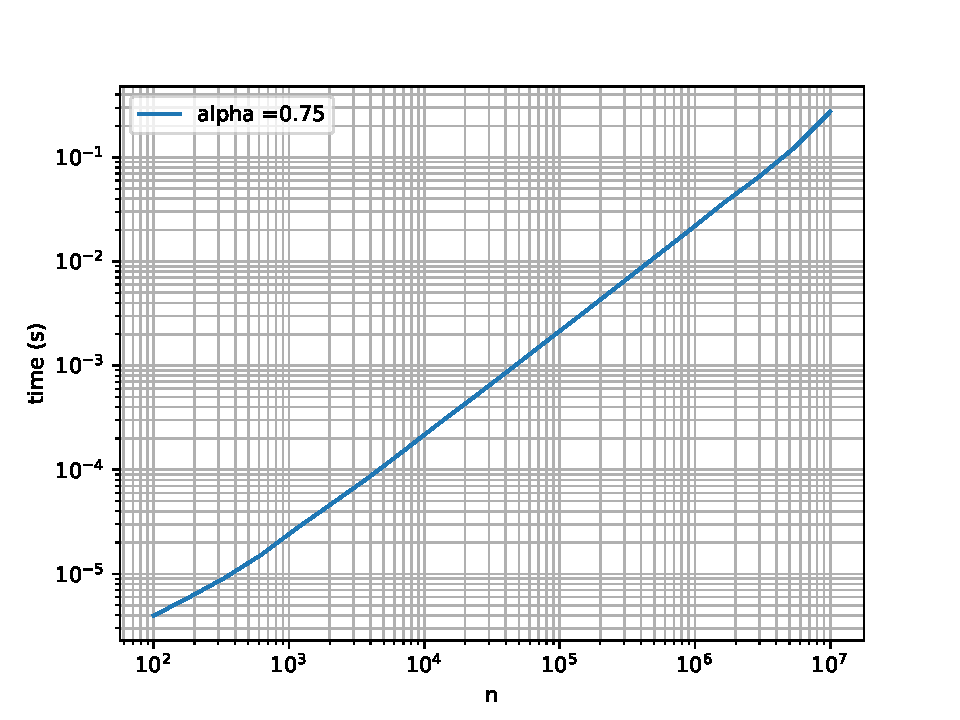
\includegraphics[width = \columnwidth]{t_time.pdf}
\end{figure}

\subsection{Quadratic Time Algorithm}

\subsection{Quasilinear time problem decomposition}

\subsection{Efficient Implementation}


\section{Sliced Partial Transport}


\section{Results}

\subsection{Algorithm efficiency}

\subsection{Color Transfer}

\subsection{Point Cloud Registration}
        

\bigskip

%\addsec{Conclusion}
\section*{Conclusion}


\section*{Remerciements}


\bibliographystyle{unsrt}
\bibliography{bibli}

\end{document}
